\documentclass{beamer}
% From share latex templates  - default presentation 
% Choose how your presentation looks.
%
% For more themes, color themes and font themes, see:
% http://deic.uab.es/~iblanes/beamer_gallery/index_by_theme.html
%
\mode<presentation>
{
  \usetheme{Boadilla}      % or try Darmstadt, Madrid, Warsaw, ...
  \usecolortheme{owl} % or try albatross, beaver, crane, ...
  \usefonttheme{serif}  % or try serif, structurebold, ...
   \setbeamertemplate{navigation symbols}{}
  \setbeamertemplate{caption}[numbered]
} 

\usepackage{tikz}
\usepackage{tikz}
\usepackage{graphicx}
\newcommand*{\ClipSep}{0.09cm}%
\newcommand{\rlogo}[3]{%
\begin{tikzpicture}
\node [inner sep=#1] at (0,0) {\includegraphics[width=#2]{#3}};
\draw [white, rounded corners=\ClipSep, line width=\ClipSep] 
    (current bounding box.north west) -- 
    (current bounding box.north east) --
    (current bounding box.south east) --
    (current bounding box.south west) -- cycle
    ;
\end{tikzpicture}}

\newcommand{\mylogo}[3]{%
	\tikz\node[draw,thick,inner sep=2pt,rounded corners=#1,text=white,path picture={\node at (path picture bounding box.center){\includegraphics[width=#2]{#3}};}]{};
}%
\usepackage[percent]{overpic}
\usepackage[english]{babel}
\usepackage[utf8x]{inputenc}
\usepackage{fontspec}
\setmainfont{Michroma}
%\setmainfont{Courier}
\usebackgroundtemplate%
{%
    
\includegraphics[width=\paperwidth,height=\paperheight]{./back_net.jpg}%
}

\makeatletter
\gdef\@ptsize{2} % 1 for 11pt doc, 2 for 12pt
\makeatother
\usepackage{setspace}
\doublespace

\title[Linux: Get Your Feet Wet]{Linux : Get your feet wet}
\author{Bridge Course '19}
\institute{EE Dept IITB}
\date{24 July 2019}

\begin{document}

\begin{frame}
\begin{center}

\includegraphics[scale=0.5]{./gnome_logo.png}%
\end{center}
\titlepage
\end{frame}

% Uncomment these lines for an automatically generated outline.
\begin{frame}{Outline}
  \tableofcontents
\end{frame}

\section{Introduction}
\subsection{What is Linux}


\begin{frame}
\textbf{Linux is a family of open source Unix-like operating systems based on the Linux kernel, Typically packaged in a Linux distribution}
\vskip 1cm
\rlogo{1pt}{2.0cm}{./ubuntu.png}
\rlogo{1pt}{2.0cm}{./centos.png}
\rlogo{1pt}{2.0cm}{./fedora.jpeg}
\rlogo{1pt}{2.0cm}{./arch.jpeg}
\rlogo{1pt}{2.0cm}{./lubuntu.png}
\newline
\rlogo{1pt}{2.0cm}{./rhel.png}
\rlogo{1pt}{2.0cm}{./kali3.jpeg}
\rlogo{1pt}{2.0cm}{./debian.png}
\rlogo{1pt}{2.0cm}{./mate.png}
\rlogo{1pt}{2.0cm}{./suse.png}
%\begin{block}{Examples}
%Some examples of commonly used commands and features are included, to help you get started.
%\end{block}

\end{frame}
\subsection{Why Linux}
\begin{frame}{Why Linux}
\begin{enumerate}
	\item<2-> Access to hardware - almost no restrictions
	\item<3-> Opensource - view code , modify , learn create
	\item<4-> Tailor Made - servers , fedora scientific
	\item<5-> Top 100 fastest supercomputers run linux 
	\item<6-> Almost all tech giants funds linux development
\end{enumerate}
\end{frame}
\begin{frame}{Why Linux ctd..}
\begin{enumerate}
	\item<2-> Free
	\item<3-> Sabko Cadence chalana he
	\item<4-> Friends urge friends to use windows 
	\item<5-> Microsoft gives you windows. Linux gives you whole house
\end{enumerate} 
\end{frame}
\section{Linux Basics}
\subsection{Linux File System}
{
	%\usebackgroundtemplate%
	%{%
	 %   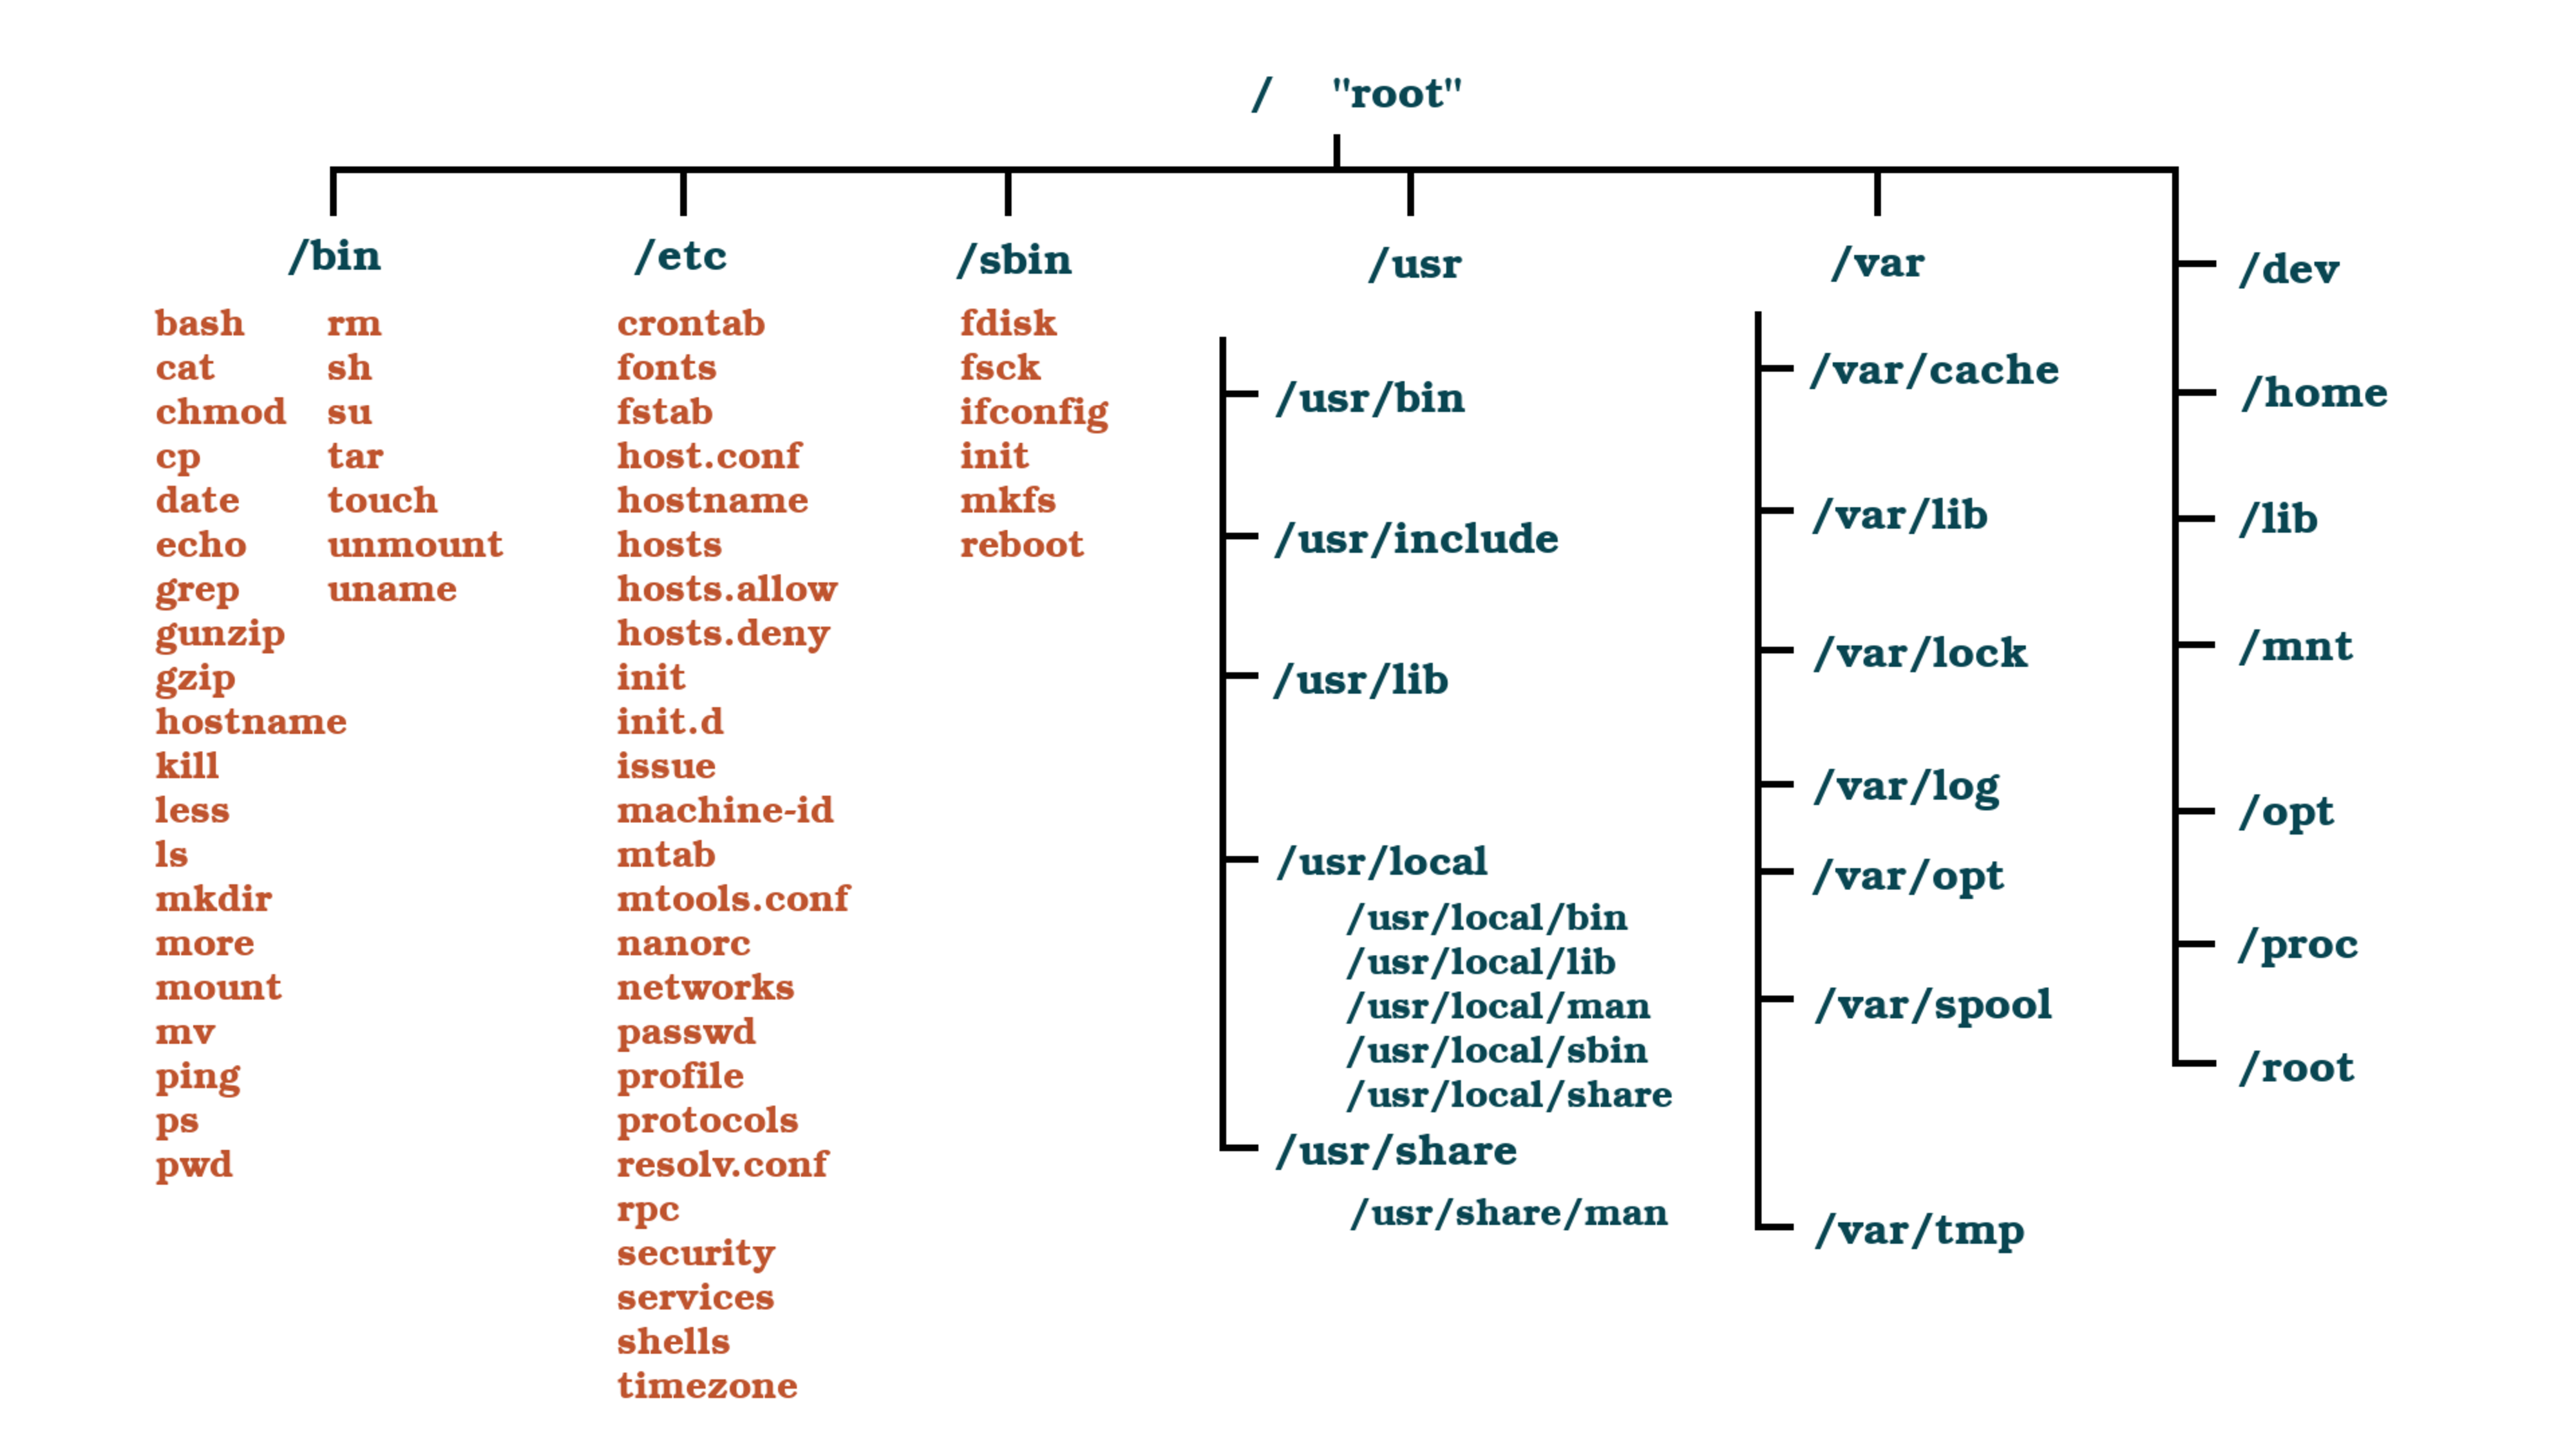
\includegraphics[height=0.8\textheight]{./filesystem.pdf}%
	%}

	\begin{frame}{File System Hierarchy}
		\begin{figure}
			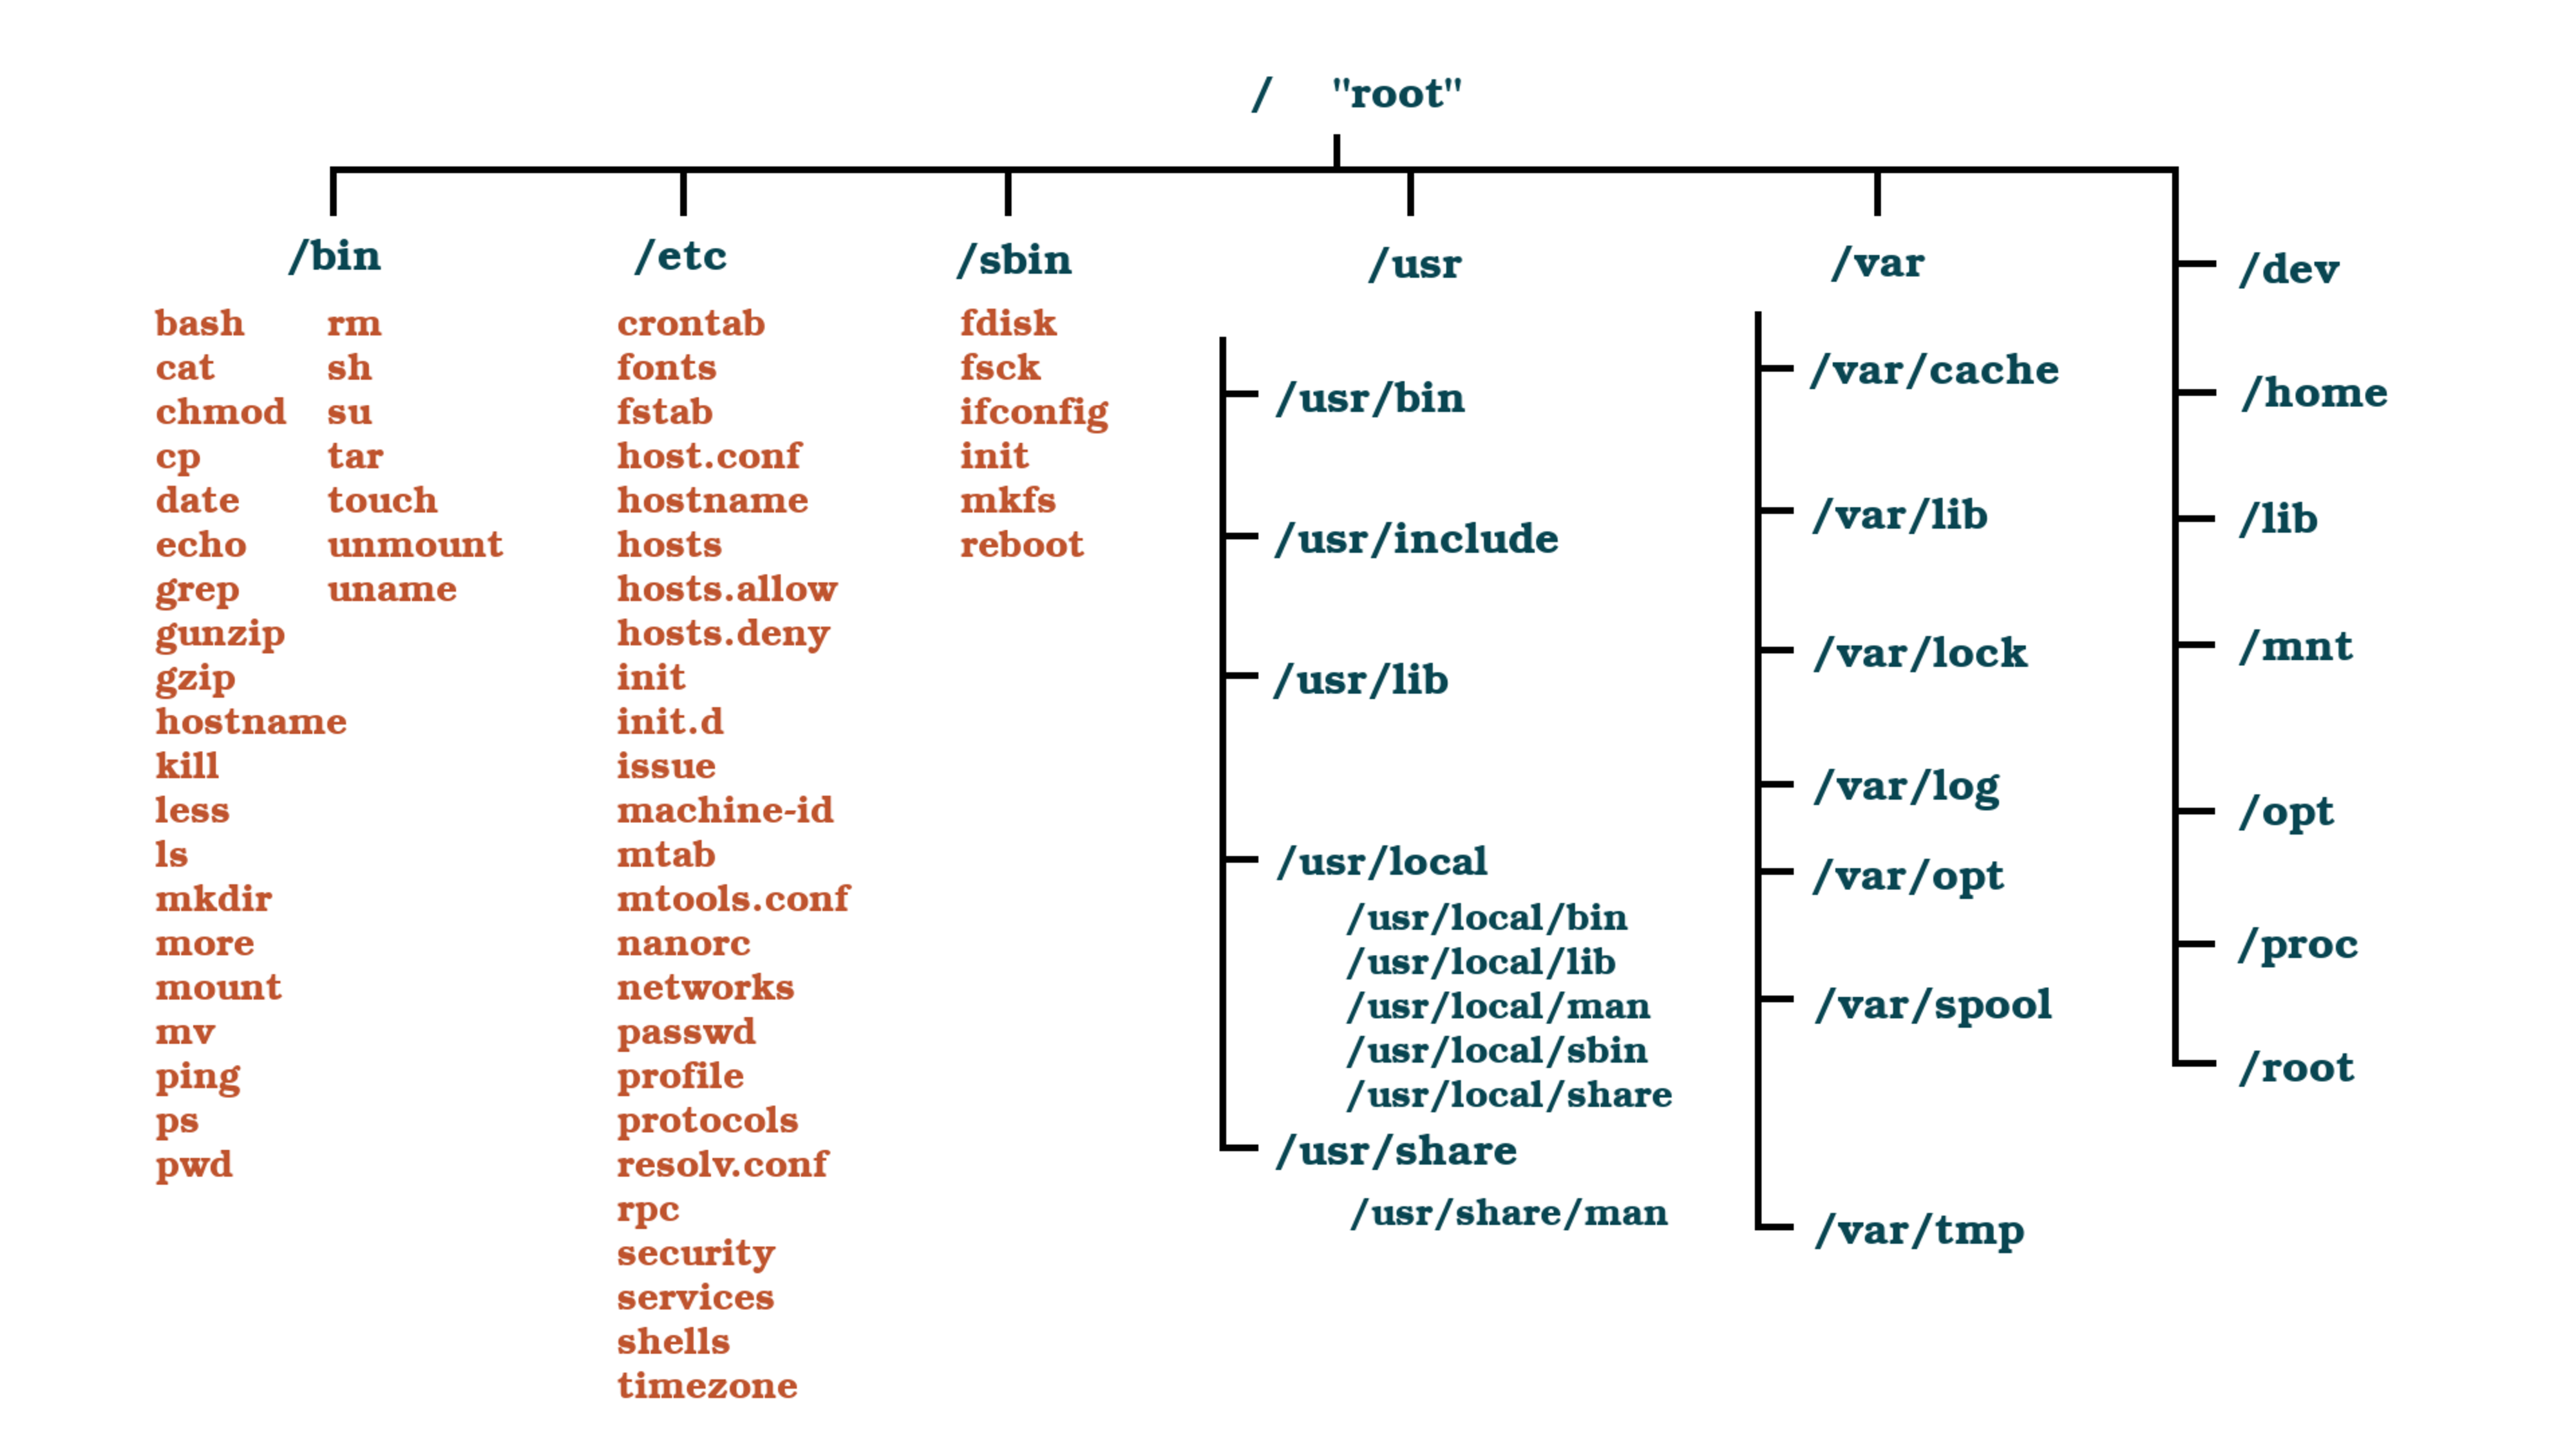
\includegraphics[width=0.9\paperwidth,height=0.8\paperheight]{./filesystem.pdf}
		\end{figure}
	\end{frame}
}

{\fontfamily{Serif}\selectfont
\begin{frame}{Linux File System:  Basic commands}
\begin{enumerate}
	\item<2->ls  - list the files the current directory
	\item<3->pwd - print the working directory
	\item<4->touch <file\_name> - create an empty file 
	\item<5->mkdir <dir\_name> - create a directory
	\item<6->cd 	- change directory 
\end{enumerate}
	\begin{alertblock}{Note}
		{use : man <command> - to get the full details regarding any command }
	\end{alertblock}
\end{frame}
}
{
	\usebackgroundtemplate%
	{%
	    
\includegraphics[width=\paperwidth,height=\paperheight]{./back_net.jpg}%
	}
\fontfamily{Serif}\selectfont
\begin{frame}{Users, Group and Permissions}
	As we saw, everything can be treated as a file in linux. \\
	\pause
	Who has permissions to edit these files???\\
	\pause
	For each file, linux assigns a set of attributes , some of these decides which users can {\textbf{Read , Write}} and (if possible )\textbf{Execute} the file. These attributes are called the file permissions. \\
	\pause
	For each file, permissions are given in three categories.
			
\end{frame}
\begin{frame}{Users, Group and Permissions}
\begin{center}
		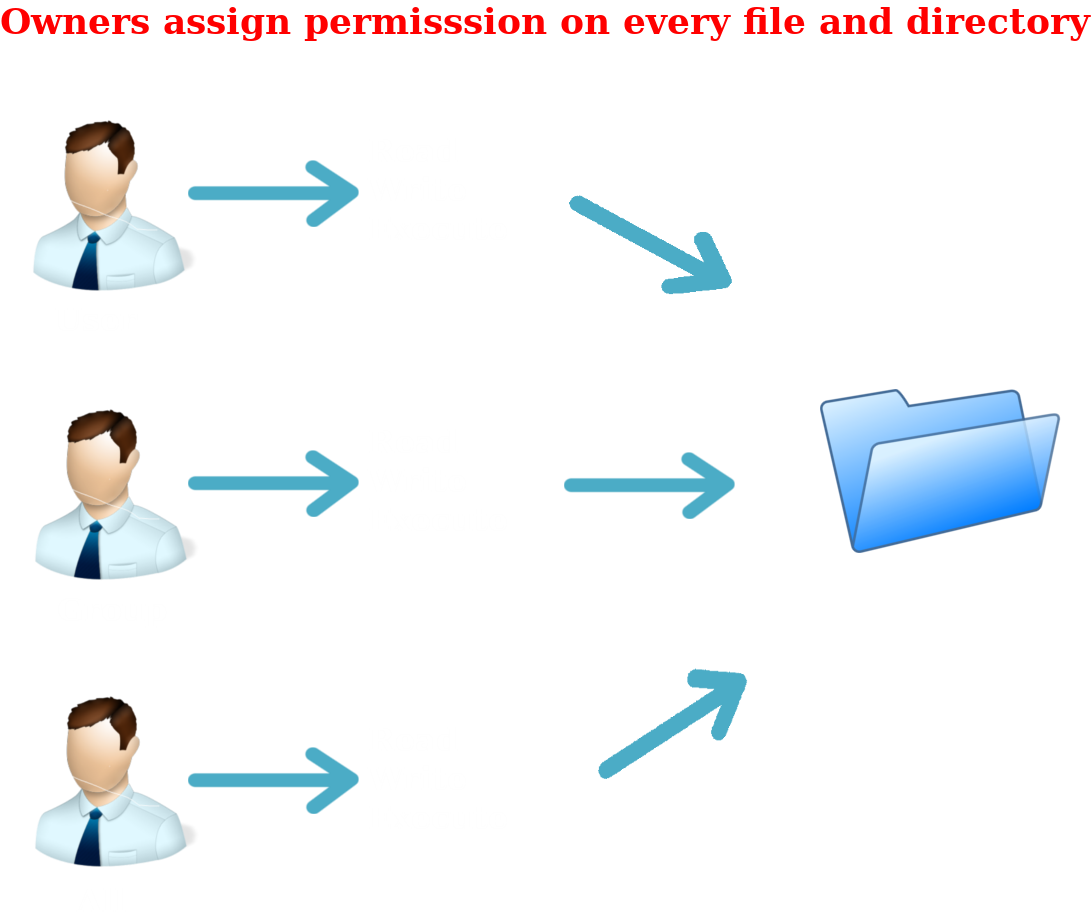
\includegraphics[scale=0.16]{./file_permissions2.png}%

%	\vskip 1cm
			USER|GROUP|ALL . \\
			 RWX-RWX-RWX\\
\end{center}

			
\end{frame}
}
\section{Some \LaTeX{} Examples}

\subsection{Tables and Figures}

\begin{frame}{Tables and Figures}

\begin{itemize}
\item Use \texttt{tabular} for basic tables --- see Table~\ref{tab:widgets}, for example.
\item You can upload a figure (JPEG, PNG or PDF) using the files menu. 
\item To include it in your document, use the \texttt{includegraphics} command (see the comment below in the source code).
\end{itemize}

% Commands to include a figure:
%\begin{figure}
%\includegraphics[width=\textwidth]{your-figure's-file-name}
%\caption{\label{fig:your-figure}Caption goes here.}
%\end{figure}

\begin{table}
\centering
\begin{tabular}{l|r}
Item & Quantity \\\hline
Widgets & 42 \\
Gadgets & 13
\end{tabular}
\caption{\label{tab:widgets}An example table.}
\end{table}

\end{frame}

\subsection{Mathematics}

\begin{frame}{Readable Mathematics}

Let $X_1, X_2, \ldots, X_n$ be a sequence of independent and identically distributed random variables with $\text{E}[X_i] = \mu$ and $\text{Var}[X_i] = \sigma^2 < \infty$, and let
$$S_n = \frac{X_1 + X_2 + \cdots + X_n}{n}
      = \frac{1}{n}\sum_{i}^{n} X_i$$
denote their mean. Then as $n$ approaches infinity, the random variables $\sqrt{n}(S_n - \mu)$ converge in distribution to a normal $\mathcal{N}(0, \sigma^2)$.

\end{frame}

\end{document}

